\documentclass{standalone}

\usepackage{tikz}
\usepackage{amsmath}

\newcommand{\Omegahat}{\boldsymbol{\mathrm{\Omega}}}
\newcommand{\ud}{\mathop{}\!\mathrm{d}} % upright derivative symbol
\newcommand{\paren}[1]{\left( #1 \right)}

\begin{document}
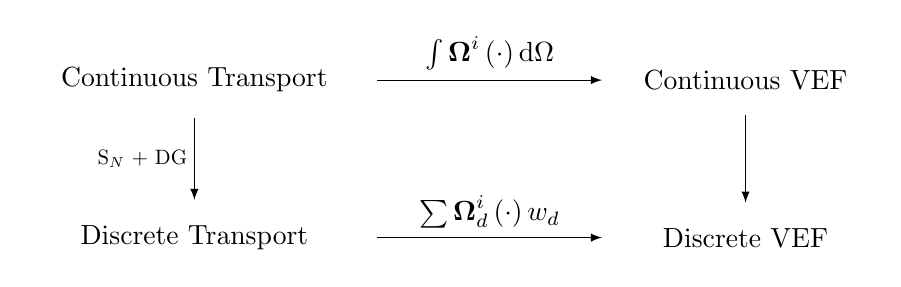
\begin{tikzpicture}[>=latex, shorten <=2mm, shorten >=2mm]
	\node[text width=4cm, text centered] (cts_trans) at (0,0) {Continuous Transport}; 
	\node[text width=4cm, text centered] (disc_trans) at (0,-2) {Discrete Transport}; 
	\node[text width=3cm, text centered] (cts_vef) at (7,0) {Continuous VEF}; 
	\node[text width=3cm, text centered] (disc_vef) at (7,-2) {Discrete VEF}; 
	\draw[->] (cts_trans) -- node[above] {$\int \Omegahat^i \paren{\cdot} \ud \Omega$} (cts_vef); 
	\draw[->] (cts_trans) -- node[left, scale=.75] {S$_N$ + DG} (disc_trans); 
	\draw[->] (disc_trans) -- node[above] {$\sum \Omegahat_d^i \paren{\cdot} w_d$} (disc_vef); 
	\draw[->] (cts_vef) -- node (pos) {} (disc_vef); 
\end{tikzpicture}
\end{document}